% Это основная команда, с которой начинается любой \LaTeX-файл. Она отвечает за тип документа, с которым связаны основные правил оформления текста.
\documentclass{article}
\usepackage[colorlinks=true, allcolors=blue]{hyperref}
\usepackage{tikz}
\usetikzlibrary{shapes.geometric, arrows.meta, positioning, calc}
\usepackage{float}
% Здесь идет преамбула документа, тут пишутся команды, которые настраивают LaTeX окружение, подключаете внешние пакеты, определяете свои команды и окружения. В данном случае я это делаю в отдельных файлах, а тут подключаю эти файлы.

% Здесь я подключаю разные стилевые пакеты. Например возможности набирать особые символы или возможность компилировать русский текст. Подробное описание внутри.
\usepackage{packages}
\usepackage{hyperref}
\usepackage[framemethod=TikZ]{mdframed}

% Здесь я определяю разные окружения, например, теоремы, определения, замечания и так далее. У этих окружений разные стили оформления, кроме того, эти окружения могут быть нумерованными или нет. Все подробно объяснено внутри.
\usepackage{environments}

% Здесь я определяю разные команды, которых нет в LaTeX, но мне нужны, например, команда \tr для обозначения следа матрицы. Или я переопределяю LaTeX команды, которые работают не так, как мне хотелось бы. Типичный пример мнимая и вещественная часть комплексного числа \Im, \Re. В оригинале они выглядят не так, как мы привыкли. Кроме того, \Im еще используется и для обозначения образа линейного отображения. Подробнее описано внутри.
\usepackage{commands}

% Потребуется для вставки картинки подписи
% \usepackage{graphicx}

% Пакет для титульника проекта
\usepackage{titlepage}

% Здесь задаем параметры титульной страницы
\setUDK{}
% Выбрать одно из двух
\setToResearch
%\setToProgram

\setTitle{Чат-бот для абитуриентов}

% Выбрать одно из трех:
% КТ1 -- \setStageOneлшшг
% КТ2 -- \setStageTwo
% Финальная версия -- \setStageFinal
% \setStageOne
% \setStageTwo
\setStageFinal

\setGroup{2412}
% Сюда можно воткнуть картинку подписи с помощью 
% \includegraphics[scale=0.2]{подпись.jpeg}
% (scale подбирается индивидуально для конкретной картинки)
\setStudentSgn{\raisebox{-4mm}{\includegraphics[scale=0.2]{подпись.jpeg}}}
\setStudent{А.В.Веляев}
\setStudentDate{11.05.2026}
\setAdvisor{Андреева Дарья Александровна}
\setAdvisorTitle{Старший инженер нейронных сетей}
\setAdvisorAffiliation{ООО "ИТ ИКС 5 ТЕХНОЛОГИИ"}
\setAdvisorDate{}
\setGrade{}
% Сюда можно воткнуть картинку подписи с помощью \includegraphics[scale=0.2]{<имя файла>}
% (scale подбирается индивидуально для конкретной картинки)
\setAdvisorSgn{}
\setYear{2026}


% С этого момента начинается текст документа
\begin{document}

% Эта команда создает титульную страницу
\makeTitlePage

% Здесь будет автоматически генерироваться содержание документа
\tableofcontents
\newpage

% Данное окружение оформляет аннотацию: краткое описание текста выделенным абзацем после заголовка
\begin{abstract}
В данной работе представлена разработка и оценка Telegram-бота для автоматизации
консультирования абитуриентов факультета компьютерных наук НИУ ВШЭ. Система
построена на основе расширенного RAG-пайплайна (Retrieval-Augmented Generation)
с многоуровневой обработкой запросов: детерминированное переформулирование,
LLM-декомпозиция на подзапросы, векторный поиск в ChromaDB с эмбеддингами
multilingual-E5, переранжирование cross-encoder'ом и генерация ответа моделью
YandexGPT. Для снижения нагрузки на языковую модель реализован трёхуровневый
FAQ-кеш с точным, нечётким и динамическим сопоставлением, который автоматически
пополняется ответами, подтверждёнными пользователями, и очищается от
некачественных записей.
Качество системы оценено на тестовом наборе вопросов по метрикам Hit@5, MRR@5,
Precision@5, Context Recall и ROUGE-L. Результаты подтверждают эффективность
предложенного подхода для задач предметно-ориентированного консультирования.

\noindent \textbf{Ключевые слова:} RAG, векторный поиск, ChromaDB, multilingual-E5,
cross-encoder, переранжирование, декомпозиция запросов, YandexGPT,
Telegram-бот, НИУ ВШЭ.
\end{abstract}
\newpage


\section{Введение}

В последнее десятилетие большие языковые модели (LLM) стали активно применяться
для автоматизации пользовательских коммуникаций. В образовательной среде это
направление особенно актуально: университеты ежегодно обрабатывают тысячи
однотипных обращений абитуриентов, значительная часть которых поступает в сжатые
сроки приёмной кампании.
Факультет компьютерных наук НИУ ВШЭ в пиковые периоды сталкивается с резким
ростом числа запросов к учебному офису. Традиционный подход~--- самостоятельное
изучение объёмных нормативных документов~--- снижает оперативность получения
информации и увеличивает нагрузку на сотрудников. При этом применение «чистых»
LLM без привязки к актуальной документации сопряжено с риском галлюцинаций~---
генерации правдоподобных, но фактически недостоверных ответов.
Целью данной работы является проектирование и реализация чат-бота на базе
архитектуры Retrieval-Augmented Generation (RAG), ориентированного на консультирование
абитуриентов ФКН. Система предоставляет ответы, основанные исключительно на
официальных документах факультета, что позволяет минимизировать риск недостоверной
информации. Для повышения качества поиска применяются многоуровневое
переформулирование запросов, векторный поиск с эмбеддингами multilingual-E5,
переранжирование cross-encoder'ом и трёхуровневый FAQ-кеш.
В работе описаны архитектурные решения системы, принципы формирования базы
знаний, а также результаты оффлайн-оценки качества на тестовом
наборе вопросов по метрикам Hit@5, MRR@5, Precision@5, Context Recall и ROUGE-L.


\noindent 
\subsection{Актуальность}
\noindent
Рост числа обращений абитуриентов в периоды приёмных кампаний создаёт значительную нагрузку на учебные офисы и снижает оперативность предоставления ответов. Только в Telegram-чате «ФКН ПМИ 2025» было задано почти 1000 вопросов по поступлению. Учебный офис, ввиду своей нагрузки, не всегда мог быстро ответить на вопрос, так как требовалось проверять информацию в нормативных документах. Поэтому, чтобы уменьшить время ожидания ответа, а также снизить нагрузку на сотрудников, целесообразно использовать чат-бота, который обеспечивает мгновенную обратную связь и удобен для пользователей. 


\subsection{Цели и задачи}

\noindent\textbf{Цель работы} --- разработка и оценка интеллектуальной системы
консультирования абитуриентов ФКН НИУ ВШЭ на основе архитектуры RAG,
обеспечивающей достоверные ответы исключительно из официальных документов
в режиме 24/7.

\noindent\textbf{Задачи:}
\begin{enumerate}
    \item Проанализировать существующие подходы к построению RAG-систем и
    обосновать выбор архитектурных решений для предметно-ориентированного
    консультирования.

    \item Собрать и структурировать базу знаний из официальных документов
    факультета, обеспечив её полноту и актуальность для нужд приёмной кампании.

    \item Исследовать методы улучшения качества поиска~--- переформулирование
    и декомпозицию запросов, переранжирование~--- и реализовать их в рамках
    единого пайплайна.

    \item Разработать механизм кеширования, снижающий зависимость системы
    от языковой модели при обработке повторяющихся запросов.

    \item Реализовать пользовательский интерфейс, обеспечивающий безопасное
    и удобное взаимодействие с системой в мессенджере Telegram.

    \item Провести количественную оценку качества системы и сравнить
    эффективность отдельных компонентов пайплайна.
\end{enumerate}


\section{Обзор литературы}
Разработка систем автоматического ответа на вопросы пользователей представляет собой активно развивающуюся область исследований, в которой сложились несколько принципиально различных подходов. В данном разделе рассматриваются основные из них применительно к задаче настоящего проекта~--- созданию чат-бота для ответов на вопросы абитуриентов НИУ ВШЭ на основе официальных документов.
\subsection{Подходы к построению вопросно-ответных систем}
Исторически первым решением стали кнопочные боты с фиксированными сценариями. Несмотря на детерминированность и легкость проверки, они принципиально ограничены невозможностью обработки произвольных запросов и необходимостью ручной переработки при любом изменении данных.Современные исследования в области обработки естественного языка (NLP) предлагают два концептуально различных подхода к интеграции внешних знаний в большие языковые модели (LLM).

\noindent Первый из них --- \textbf{дообучение (Fine-tuning)} --- предполагает адаптацию предобученной модели под специфику конкретной предметной области путём дополнительного обучения на собственных данных. Однако данный подход сопряжён со значительными практическими трудностями. Современные языковые модели обучаются на колоссальных объёмах данных с применением сложной инфраструктуры и множества оптимизаций, без которых корректно встроить новые знания крайне затруднительно. Помимо высоких требований к вычислительным ресурсам и экспертизе, метод обладает и структурным недостатком: знания модели остаются статичными на момент обучения, а любое обновление нормативной документации требует полного цикла переобучения. В условиях регулярно актуализируемых правил приёма это делает дообучение практически неприменимым.
Второй подход --- \textbf{Retrieval-Augmented Generation (RAG)} --- строится на принципиально иной логике: модель не заучивает факты на этапе обучения, а динамически извлекает их из внешнего хранилища в момент обработки запроса. Входной запрос пользователя преобразуется в векторное представление (эмбеддинг), на основе которого система осуществляет семантический поиск и отбирает релевантные фрагменты документов. Сформированный контекст передаётся языковой модели, которая синтезирует на его основе итоговый ответ. Такой подход обеспечивает актуальность информации: обновление базы знаний не требует переобучения и сводится к замене или дополнению документов в хранилище.

% Альтернативой выступает «закрытый» генеративный подход, где модель опирается только на знания, заложенные при обучении. Для задач, требующих точного следования регламентам университета, такой подход недостаточен, так как модель не имеет доступа к актуальным локальным актам и склонна генерировать правдоподобные, но неверные утверждения.
% Принципиальным решением стала архитектура
% \textit{Retrieval-Augmented Generation} (RAG) \cite{6}. Она сочетает генеративные способности LLM с внешним хранилищем документов. На каждый запрос система извлекает релевантные фрагменты текста и подает их модели в качестве контекста. Это обеспечивает строгую привязку ответа к источникам и позволяет обновлять базу знаний без переобучения нейросети.



\subsection{Обоснование выбора RAG}
С учётом требований и ограничений настоящего проекта архитектура RAG представляется наиболее обоснованным техническим решением. Концепция RAG была формализована в работе Lewis et al. \cite{1}, где авторы показали, что модели, сочетающие параметрическую и непараметрическую память, генерируют более точные и фактически достоверные ответы по сравнению с системами, опирающимися исключительно на веса модели. Как отмечается в обзоре Gao et al. \cite{3}, ключевыми проблемами современных языковых моделей являются именно галлюцинации, устаревание знаний и непрозрачность рассуждений --- RAG выступает признанным решением каждой из них.Прежде всего, система должна оперировать исключительно официальными документами \href{https://ba.hse.ru/docs}{НИУ ВШЭ}, не допуская генерации ответов на основе параметров модели. Это обусловлено высокой ценой ошибки: сведения о сроках подачи документов, условиях поступления и требованиях к абитуриентам носят юридически значимый характер, и любое фактическое искажение --- так называемая «галлюцинация» модели --- может повлечь за собой серьёзные последствия для пользователя. RAG устраняет данный риск, привязывая каждый ответ к конкретному фрагменту источника.
Помимо этого, нормативная документация приёмной кампании регулярно обновляется. В отличие от дообучения, архитектура RAG позволяет актуализировать информационную базу без какого-либо вмешательства в параметры модели --- достаточно обновить документы в хранилище.
Совокупность указанных факторов определила выбор RAG в качестве архитектурной основы разрабатываемой системы. 

\newpage

\section{Архитектура системы}


\noindent Реализованная система представляет собой расширенный RAG-пайплайн,
сочетающий два дополняющих друг друга метода улучшения запроса: переформулирование (Query Rewriting) и декомпозицию (Query Decomposition). Необходимость такого подхода обусловлена семантическим разрывом между разговорным стилем пользовательских запросов и официально-деловым регистром нормативных документов. Как показано в работе~\cite{2}, прямой поиск по исходному запросу систематически уступает подходу «переформулировать~--- извлечь~--- ответить» (Rewrite-Retrieve-Read), поскольку позволяет привести запрос к семантическому пространству базы знаний.Обработка запроса выполняется в два последовательных этапа. На первом этапе применяется детерминированное лексическое переформулирование на основе регулярных выражений для нормализации студенческого сленга. На втором этапе языковая модель YandexGPT одновременно переформулирует запрос и разбивает его на подзапросы. Данная стратегия декомпозиции опирается на метод Multi-Query Retrieval, который эффективно решает проблему чувствительности эмбеддингов к точным формулировкам, генерируя различные семантические вариации одного вопроса.Для каждого подзапроса выполняется независимый поиск в векторном хранилище ChromaDB. Использование модели \mbox{multilingual-E5} обосновано её высокой производительностью в задачах извлечения текстов на разных языках, подтвержденной в сравнительных бенчмарках~\cite{4}. Полученные чанки объединяются и дедуплицируются. Критически важным этапом является переранжирование (Reranking). Согласно экспериментальному исследованию ARAGOG~\cite{5}, использование внешних реранкеров является наиболее эффективным методом повышения точности (Precision) RAG-систем. Применение Cross-Encoder архитектуры позволяет более детально оценить релевантность фрагмента контекста за счёт механизма полного внимания между токенами вопроса и документа~\cite{6}, что нивелирует недостатки стандартного косинусного сходства векторов. Итоговый контекст передаётся в генеративную модель для формирования финального ответа.


\bigskip
\bigskip


\begin{figure}[H]
\centering
\resizebox{\linewidth}{!}{%
\begin{tikzpicture}[
  node distance = 2.2cm and 2.5cm,
  user/.style   = {draw, ellipse,
                   fill=orange!25, draw=orange!70!black,
                   minimum height=0.9cm, minimum width=2.2cm,
                   align=center, font=\small\bfseries\sffamily},
  process/.style= {draw, rectangle, rounded corners=5pt,
                   fill=blue!8, draw=blue!50!black,
                   minimum height=1.3cm, minimum width=3.8cm,
                   align=center, font=\small\sffamily},
  preproc/.style= {draw, rectangle, rounded corners=5pt,
                   fill=yellow!15, draw=yellow!60!black,
                   minimum height=1.0cm, minimum width=3.2cm,
                   align=center, font=\small\sffamily},
  interim/.style= {draw, rectangle, rounded corners=5pt, dashed,
                   fill=gray!6, draw=gray!55,
                   minimum height=1.0cm, minimum width=2.8cm,
                   align=center, font=\small\itshape\sffamily},
  db/.style     = {draw, cylinder, cylinder uses custom fill,
                   cylinder body fill=green!10, cylinder end fill=green!25,
                   draw=green!50!black, shape border rotate=90,
                   minimum height=1.4cm, minimum width=2.2cm,
                   align=center, font=\small\sffamily},
  arr/.style    = {-{Latex[length=6pt]}, thick, draw=gray!60},
  arrD/.style   = {-{Latex[length=6pt]}, thick, dashed, draw=gray!50},
  lbl/.style    = {font=\fontsize{7}{8}\selectfont\itshape,
                   align=center, text=gray!70!black,
                   inner sep=1.5pt}
]

%── Ряд 1 (Вход -> Rewriting -> Decomposition) ───────────────────────────
\node[user] (user_in) {Пользователь};

\node[preproc, right=1.6cm of user_in] (rewrite)
  {\textbf{Query Rewriting}\\[2pt]
   {\fontsize{7}{8}\selectfont\itshape (Regex normalization)}};

\node[process, right=1.6cm of rewrite] (decompose)
  {\textbf{YandexGPT}\\[2pt]
   Query Decomposition};

\node[interim, right=1.6cm of decompose] (sub_q)
  {подзапрос$_1$, \dots, подзапрос$_3$\\[2pt]
   (Multi-Query)};

%── Переход вниз ──────────────────────────────────────────────────────────
\node[process, below=2.5cm of sub_q] (retrieval)
  {\textbf{multilingual-E5}\\[1pt]
   \textbf{+ ChromaDB}\\[2pt]
   Retrieval};

\node[db, below=1.5cm of retrieval] (docs) {База знаний};

%── Ряд 2 (справа налево: Rerank -> Generation) ───────────────────────────
\node[process, left=of retrieval] (rerank)
  {\textbf{Cross-Encoder}\\[2pt]
   {\fontsize{7}{8}\selectfont\itshape Reranking}};

\node[process, left=of rerank] (generation)
  {\textbf{YandexGPT}\\[2pt]
   Generation};

%── Выход ─────────────────────────────────────────────────────────────────
\node[user, below=2.0cm of generation] (user_out) {Пользователь};

%── Стрелки ───────────────────────────────────────────────────────────────

\draw[arr] (user_in) -- 
  node[lbl, above, yshift=2pt] {исходный} 
  node[lbl, below, yshift=-2pt] {вопрос} 
  (rewrite);

\draw[arr] (rewrite) -- 
  node[lbl, above, yshift=2pt] {} 
  node[lbl, below, yshift=-2pt] {} 
  (decompose);

\draw[arr] (decompose) -- (sub_q);

\draw[arr] (sub_q) --
  node[lbl, right, xshift=5pt] {векторные\\запросы}
  (retrieval);

\draw[arr] (retrieval.290) -- node[lbl, right, xshift=5pt] {поиск} (docs.70);
\draw[arrD] (docs.110) -- node[lbl, left, xshift=-5pt] {чанки} (retrieval.250);

\draw[arr] (retrieval) --
  node[lbl, above, yshift=2pt] {объединённые}
  node[lbl, below, yshift=-2pt] {чанки}
  (rerank);

\draw[arr] (rerank) --
  node[lbl, above, yshift=2pt] {контекст}
  node[lbl, below, yshift=-2pt] {+ вопрос}
  (generation);

\draw[arr] (generation) --
  node[lbl, right, xshift=5pt] {финальный\\ответ}
  (user_out);

\end{tikzpicture}%
}
\caption{Схема работы RAG-системы с переформулированием и декомпозицией запроса}
\label{fig:rag_scheme}
\end{figure}
\newpage
\section{Ход работы}

В данном разделе описывается процесс практической реализации системы. Работа разделена на несколько ключевых этапов: подготовка корпуса знаний, выбор и настройка модели векторных представлений, построение индексного хранилища, реализация многостадийного retrieval-пайплайна и его интеграция с большой языковой моделью. 



\subsection{Описание датасетов}

\subsubsection{База знаний}

База знаний сформирована из 13 тематических документов в формате Markdown
общим объёмом около 138\,000 символов. Каждый документ охватывает одну
предметную область, что позволяет контролировать полноту покрытия тем.
Структура базы знаний представлена в таблице.

\begin{table}[h]
\centering
\begin{tabular}{lll}
\hline
\textbf{Файл} & \textbf{Тема} & \textbf{Тип} \\
\hline
fkn\_programs\_rag.md       & Программы и минимальные баллы ЕГЭ & Нормативный \\
fkn\_achievements\_rag.md   & Индивидуальные достижения          & Нормативный \\
fkn\_discounts\_rag.md      & Скидки на обучение                 & Нормативный \\
fkn\_dormitory\_rag.md      & Общежитие                          & Нормативный \\
fkn\_contract\_rag.md       & Договор об оказании услуг          & Нормативный \\
fkn\_military\_rag.md       & Военная кафедра                    & Нормативный \\
fkn\_academic\_process\_rag.md & Академический процесс           & Нормативный \\
fkn\_foreign\_rag.md        & Иностранные граждане               & Нормативный \\
fkn\_ovz\_rag.md            & Абитуриенты с ОВЗ                  & Нормативный \\
fkn\_timeline\_rag.md       & Сроки подачи документов            & Нормативный \\
fkn\_tuition\_rag.md        & Стоимость обучения                 & Нормативный \\
fkn\_summary\_rag.md        & Сводная информация по программам   & Нормативный \\
ЧАТ\_ФКН\_2025.md           & FAQ Telegram-канала ФКН            & FAQ \\
\hline
\end{tabular}
\caption{Состав базы знаний}
\label{tab:knowledge_base}
\end{table}

\noindent Документы собирались из двух источников: официальные PDF-документы НИУ ВШЭ 
(Правила приёма 2026 и приложения к ним с \href{https://ba.hse.ru}{официального сайта}) и 
Telegram-канал Студенческого совета ФКН за 2024--2026 годы. Текст извлекался 
с помощью библиотеки pdfplumber, после чего структурировался 
в формат Markdown с использованием языковой модели: нормативные 
документы приводились к иерархической разметке по разделам, а сообщения 
Telegram-канала~--- к FAQ-структуре с явным выделением вопроса и ответа. После автоматизированной обработки весь контент проходил этап ручной верификации для устранения возможных галлюцинаций модели и проверки фактической точности данных.



\subsubsection{Тестовый датасет}

Для оценки системы сформирован датасет из 300 пар «вопрос~--- эталонный
ответ». Структура каждой записи описана в таблице.

\begin{table}[h]
\centering
\begin{tabular}{llp{6cm}}
\hline
\textbf{Поле} & \textbf{Тип} & \textbf{Описание} \\
\hline
\texttt{id}         & str  & Идентификатор записи (Q01--Q300) \\
\texttt{question}   & str  & Текст вопроса пользователя \\
\texttt{answer}     & str  & Эталонный ответ из официальных документов \\
\texttt{category}   & str  & Тематическая категория (см. табл.~\ref{tab:dataset_categories}) \\
\texttt{route}      & str  & Ожидаемый маршрут: \texttt{rag}, \texttt{clarification}, \texttt{blocked},  \texttt{faq} \\
\texttt{source\_doc}& str  & Документ базы знаний, содержащий эталонный ответ \\
\hline
\end{tabular}
\caption{Поля тестового датасета}
\label{tab:dataset_fields}
\end{table}

\noindent Датасет разбит на несколько категорий, равномерно распределённых по трём частям, где каждая следующая часть
расширяет тематическое покрытие. Состав категорий приведён в
таблице.

\begin{table}[h]
\centering
\begin{tabular}{lcc}
\hline
\textbf{Тип / тема вопроса} & \textbf{Маршрут} & \textbf{Кол-во} \\
\hline
\multicolumn{3}{l}{\textit{Тематические вопросы}} \\
Программы, поступление, баллы ЕГЭ      & rag       & 26 \\
Олимпиады и индивидуальные достижения   & rag       & 25 \\
Сроки, документы, договор              & rag       & 25 \\
ОВЗ и иностранные граждане             & rag       & 30 \\
Стоимость обучения и скидки            & rag       & 24 \\
Общежитие                              & rag       & 14 \\
Военная кафедра                        & rag       & 11 \\
Академический процесс                  & rag       & 19 \\
\hline
\multicolumn{3}{l}{\textit{Специальные типы}} \\
Сленговые и разговорные формулировки   & rag       & 30 \\
Сложные и составные вопросы            & rag       & 41 \\
\hline
\multicolumn{3}{l}{\textit{Фильтруемые запросы}} \\
Грубые / нецензурные                   & blocked   & 35 \\
Офтопик-запросы                        & blocked   & 20 \\
\hline
\textbf{Итого}                         &           & \textbf{300} \\
\hline
\end{tabular}
\caption{Состав и структура тестового датасета}
\label{tab:dataset_categories}
\end{table}

\noindent Вопросы составлялись вручную на основе анализа Telegram-чатов абитуриентов
ФКН за 2024 и 2025 годы. Эталонные ответы находились в официальных
документах и фиксировались вручную. Тестовая выборка не входила в базу
знаний и использовалась исключительно для оценки. Датасет опубликован в открытом доступе в формате Markdown%
\footnote{\url{https://github.com/aveliaev/RAG_HSE}}


\subsection{Подготовка данных и метод чанкирования}

\subsubsection{Предобработка текстов}

Извлечённый из PDF-файлов «сырой» текст содержал колонтитулы, номера страниц
и артефакты переноса строк. Очистка выполнялась в два шага. На первом шаге
применялась библиотека \textit{pdfplumber}, которая корректно обрабатывает
многоколончатые таблицы и извлекает структурированный текст без артефактов
разрыва строк. На втором этапе для приведения документов к единому формату разметки Markdown использовалась большая языковая модель. На следующем этапе нормативные документы были преобразованы в иерархическую структуру с использованием заголовков уровней \texttt{\#}, \texttt{\#\#} и \texttt{\#\#\#}. Материалы Telegram-канала были трансформированы в FAQ-структуру, где вопросы выделялись полужирным начертанием, а ответы отделялись логическим разрывом строки. 
Важным этапом подготовки стала последующая ручная сверка полученных данных.

\subsubsection{Метод чанкирования}

Документы базы знаний имеют разную структуру: одни оформлены как FAQ
с явными парами «вопрос~--- ответ», другие~--- как нормативные документы
с иерархией разделов. Поэтому вместо нарезки текста на фрагменты
фиксированного размера применяется структурное чанкирование~---
разбиение по разметке документа. Это гарантирует, что каждый чанк
содержит логически завершённую мысль, а не обрывается посередине абзаца
или таблицы. Алгоритм автоматически выбирает одну из трёх стратегий в зависимости
от структуры документа.
FAQ-стратегия применяется к документам, в которых не менее пяти строк
содержат разметку жирного заголовка формата \texttt{**...**}:
каждая пара «вопрос~--- ответ» становится отдельным чанком.
Трёхуровневая стратегия используется при наличии подзаголовков
уровня \texttt{\#\#\#}: граница чанка проходит по каждому из них,
а в текст включаются заголовки верхних уровней для сохранения контекста.
Для остальных документов применяется двухуровневая стратегия ~---
разбиение по заголовкам уровня \texttt{\#\#}.
Слишком короткие чанки отбрасываются: менее~80 символов для
двухуровневой стратегии и менее~50~--- для трёхуровневой.
В результате корпус составил 216~чанков.
При загрузке в ChromaDB к каждому чанку добавляется префикс
\texttt{passage:}, а к поисковым запросам~--- \texttt{query:},
согласно рекомендации авторов модели multilingual-E5~\cite{4}.





\subsection{Выбор модели векторного представления текста}

Для формирования эмбеддингов текстовых данных из библиотеки
SentenceTransformers были рассмотрены три предобученные модели:
\textit{paraphrase-multilingual-MiniLM-L12-v2} (118\,М параметров),
\textit{intfloat/multilingual-e5-base} (278\,М параметров)
и \textit{BAAI/bge-m3} (570\,М параметров).
Сравнительный эксперимент проводился на выборке из 50~тематических
вопросов о поступлении в режиме чистого векторного поиска~---
без реранжирования и нормализации запросов~--- чтобы изолировать
вклад именно модели эмбеддингов.
В качестве метрик использовались стандартные показатели качества
информационного поиска: Hit Rate@3 и Mean Reciprocal Rank (MRR@3). Hit Rate@3 фиксирует долю запросов, для которых релевантный чанк
попадает в тройку лучших результатов; MRR@3 отражает среднюю обратную
позицию правильного чанка в ранжированной выдаче и тем самым
характеризует пригодность результатов для последующей генерации ответа
языковой моделью.

\begin{table}[H]
\centering
\begin{tabular}{lcc}
\hline
\textbf{Модель} & \textbf{Hit Rate@3} & \textbf{MRR@3} \\
\hline
paraphrase-multilingual-MiniLM-L12-v2  & 0{,}660 & 0{,}583 \\
BAAI/bge-m3                            & 0{,}740 & 0{,}671 \\
\textbf{intfloat/multilingual-e5-base} & \textbf{0{,}820} & \textbf{0{,}748} \\
\hline
\end{tabular}
\caption{Сравнение моделей векторного представления текста ($n = 50$)}
\label{tab:embed_comparison}
\end{table}

\noindent По результатам эксперимента выбрана модель \textit{intfloat/multilingual-e5-base},
показавшая наилучшие значения по обеим метрикам.
Несмотря на наибольшее число параметров, модель \textit{BAAI/bge-m3}
уступила \textit{multilingual-e5-base}: без тонкой настройки
под конкретный домен она чувствительна к формату запроса,
тогда как явные префиксы \texttt{query}/\texttt{passage}
модели E5 обеспечивают стабильное разграничение запроса и документа
на русскоязычном корпусе~\cite{4}.
Модель \textit{paraphrase-multilingual-MiniLM-L12-v2} демонстрирует
наихудшие показатели, что объясняется её меньшей размерностью
и ориентацией на задачи семантического сходства,
а не на асимметричный поиск «запрос~--- документ».

% \begin{figure}[H]  % Теперь H — это ПРИКАЗ "стоять тут"
%     \centering
%     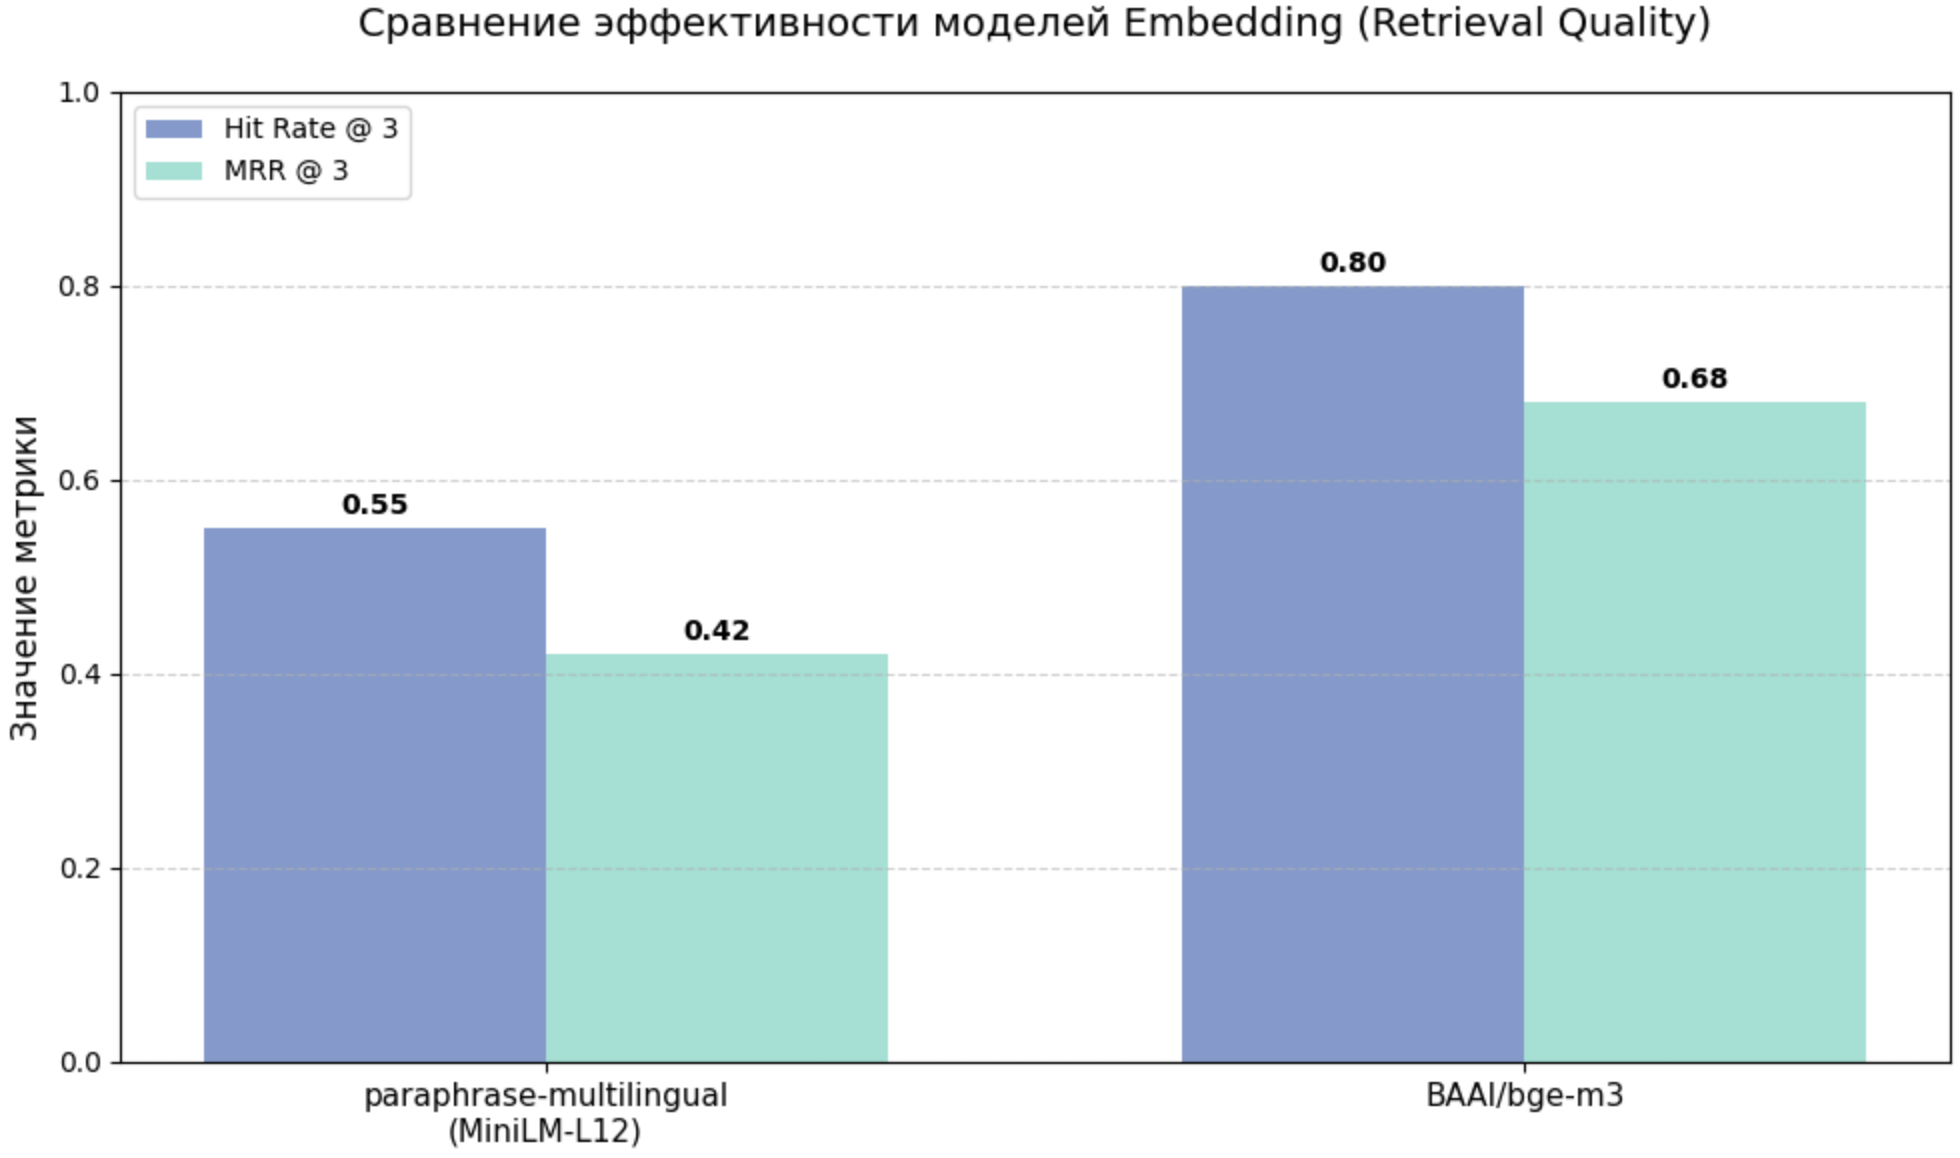
\includegraphics[width=0.7\textwidth]{график_1.png}
%     \caption{Сравнение языковой точности моделей MiniLM-L12 и BGE-M3}
%     \label{fig:comparison}
% \end{figure}

% \noindent 
% Для хранения полученных эмбеддингов и быстрого поиска по ним была выбрана векторная база данных ChromaDB \cite{2}. Данное решение было принято благодаря возможности локального хранения данных, высокой скорости семантического поиска и полной совместимости с используемой моделью эмбеддингов BGE-M3.

\subsection{Выбор модели переранжирования}

Векторный поиск на основе эмбеддингов позволяет быстро найти семантически близкие чанки, однако bi-encoder архитектура имеет принципиальное ограничение: запрос и документ кодируются независимо, без учёта их взаимного контекста. Для устранения этого недостатка в пайплайн добавлен этап переранжирования (reranking): на первом шаге векторный поиск извлекает расширенный пул кандидатов (в два раза больше целевого числа чанков), на втором шаге cross-encoder модель заново оценивает каждую пару (запрос,~чанк) совместно и переставляет кандидатов в порядке убывания релевантности. Для реализации этапа переранжирования была выбрана модель \textit{cross-encoder/mmarco-mMiniLMv2-L12-H384-v1} из библиотеки SentenceTransformers. Модель обучена на датасете mMARCO~--- многоязычной версии MS~MARCO~--- и нативно поддерживает русский язык, что критично для данной задачи. Эксперимент проводился на той же выборке из 50 вопросов; сравнивалась работа системы без переранжирования и с ним при фиксированной модели эмбеддингов \textit{multilingual-e5-base}.

\begin{table}[H]
\centering
\begin{tabular}{lcc}
\hline
\textbf{Конфигурация} & \textbf{Hit Rate@3} & \textbf{MRR@3} \\
\hline
Без переранжирования                             & 0{,}820 & 0{,}748 \\
\textbf{+ mmarco-mMiniLMv2-L12-H384-v1}         & \textbf{0{,}860} & \textbf{0{,}801} \\
\hline
\end{tabular}
\caption{Влияние переранжирования на качество поиска ($n = 50$)}
\label{tab:reranker_comparison}
\end{table}

\noindent Добавление cross-encoder reranker'а дало прирост
Hit~Rate@3  и MRR@3.
Рост MRR особенно значим: он свидетельствует о том, что релевантный
чанк стабильно поднимается на первые позиции выдачи, напрямую влияя
на качество контекста, передаваемого в генеративную модель.
Данный эффект согласуется с выводами обзора~\cite{3},
согласно которым переранжирование является одним из наиболее
эффективных методов повышения точности RAG-систем.



\subsection{Выбор метрик}

Оценка системы проводилась независимо по двум компонентам:
качеству поиска и качеству генерации ответа. Для оценки качества поиска использовались метрики
Hit@K, MRR@5, Precision@K и Context Recall.
\textbf{Hit@K} фиксирует долю запросов, для которых хотя бы один
релевантный фрагмент попал в топ-$K$ результатов.
\textbf{MRR@5} (Mean Reciprocal Rank) учитывает позицию первого
релевантного чанка, отражая стабильность ранжирования.
\textbf{Precision@K} определяет долю полезной информации
среди $K$ возвращённых фрагментов.
\textbf{Context Recall} оценивает, какая часть информации
из эталонного ответа фактически присутствует в извлечённом контексте.
Критерием релевантности чанка служила доля токенов эталонного ответа,
присутствующих в тексте фрагмента: порог составлял~$0{,}25$. Для оценки качества генерации использовались метрики семейства ROUGE.
\textbf{ROUGE-1} измеряет перекрытие униграмм между сгенерированным
и эталонным ответом, \textbf{ROUGE-L}~--- длину наибольшей общей
подпоследовательности, что позволяет учитывать порядок слов.


\subsection{Сравнительный анализ конфигураций пайплайна}

Для оценки вклада каждого компонента системы проведено накопительное
аблационное исследование: конфигурации тестируются последовательно,
каждая следующая добавляет один компонент к предыдущей.
Оценка проводилась на 245~вопросах тестового датасета (за исключением
фильтруемых запросов).
Метрики поиска вычислялись по топ-5 результатам: Hit@1, Hit@3, Hit@5,
MRR@5, Precision@3 и Context~Recall; дополнительно фиксировалась
задержка retrieval-этапа (среднее и P95).
Результаты представлены в таблице
\begin{table}[h]
\centering
\caption{Метрики качества при накопительном добавлении компонентов ($n = 245$)}
\label{tab:ablation}
\small
\begin{tabular}{lcccccccc}
\hline
\textbf{Конфигурация}
  & \textbf{Hit@1}
  & \textbf{Hit@3}
  & \textbf{Hit@5}
  & \textbf{MRR@5}
  & \textbf{P@3}
  & \textbf{CR}
  & \textbf{Lat\textsubscript{mean}}
  & \textbf{Lat\textsubscript{P95}} \\
\hline
Base RAG
  & 0{,}714 & 0{,}849 & 0{,}906 & 0{,}789 & 0{,}446 & 0{,}667
  & \textbf{16~мс} & \textbf{17~мс} \\
{+~Reranker}
  & 0{,}796 & \textbf{0{,}931} & \textbf{0{,}959} & 0{,}862 & 0{,}533 & 0{,}706
  & 234~мс & 408~мс \\
{+~Regex Rewrite}
  & \textbf{0{,}820} & 0{,}922 & 0{,}955 & \textbf{0{,}872} & \textbf{0{,}550} & 0{,}701
  & 248~мс & 462~мс \\
{+~LLM Decomp.}
  & 0{,}784 & 0{,}927 & 0{,}939 & 0{,}852 & 0{,}543 & 0{,}700
  & 1250~мс & 1707~мс \\
{+~FAQ Cache}
  & {---} & {---} & {---} & {---} & {---} & \textbf{0{,}809}
  & 786~мс & 1580~мс \\
\hline
\end{tabular}

\smallskip
\raggedright
\footnotesize
\end{table}

\noindent Retrieval-метрики для конфигурации с FAQ-кешем не применимы:
при попадании в кеш (35{,}5\% запросов) система возвращает ответ
напрямую, минуя retrieval-этап, поэтому в данном случае они
не представляют интереса.

\subsubsection{Конфигурация~1: Base RAG}

В качестве базовой конфигурации используется стандартный RAG-пайплайн~\cite{1}: пользовательский запрос напрямую передаётся в векторное хранилище ChromaDB, оснащённое эмбеддингами модели intfloat/multilingual-e5 base~\cite{4}, и возвращаются пять наиболее семантически близких фрагментов. Базовая конфигурация достигает Hit@5~$= 0.906$, что свидетельствует о том, что в 90.6\% случаев релевантный фрагмент присутствует среди  пяти возвращённых кандидатов. Вместе с тем Hit@1~$= 0.714$ указывает на существенный разрыв между первой позицией и топ-5: более чем в четверти запросов наиболее релевантный фрагмент не попадает на первое место, что снижает качество контекста, передаваемого генеративной модели. Задержка retrieval-этапа составляет 16~мс~--- наименьшая среди всех конфигураций, обусловленная компактным размером базы знаний (216~чанков).

% ─────────────────────────────────────────────────────────────────────────────
\subsubsection{Конфигурация~2: Добавление Reranker}

Основным ограничением архитектуры, лежащей в основе
векторного поиска, является раздельное кодирование запроса и документа без учёта их взаимного контекста. Для устранения этого недостатка к пайплайну добавлен этап переранжирования на основе cross-encoder модели cross-en\-co\-der/mmarco-mMiniLMv2-L12-H384-v1, обученной на многоязычной версии датасета MS~MARCO. Согласно исследованию ARAGOG~\cite{5}, применение внешних реранкеров является наиболее эффективным методом повышения точности RAG-систем. Cross-encoder оценивает каждую пару (запрос,~фрагмент) совместно через механизм полного внимания~\cite{6}, что обеспечивает более точную оценку релевантности по сравнению с косинусным сходством векторов. Добавление реранкера даёт наибольший прирост среди всех компонентов: Hit@1 вырос с~0.714 до~0.796, Hit@3~--- с~0.849 до~0.931, MRR@5~--- с~0.789 до~0.862, Precision@3~--- с~0.446 до~0.533. Платой за прирост качества стало увеличение задержки с~16 до~234~мс. Рост MRR особенно значим: он свидетельствует о том, что релевантный фрагмент стабильно поднимается на первые позиции выдачи, напрямую влияя на качество контекста для генеративной модели.

% ─────────────────────────────────────────────────────────────────────────────
\subsubsection{Конфигурация~3: Добавление Rewrite}

Ключевой проблемой при поиске по официальным нормативным документам является семантический разрыв между разговорным стилем запросов абитуриентов и официально-деловым регистром документов. Как показано в работе~\cite{2}, предварительное переформулирование запроса позволяет существенно сократить этот разрыв. В отличие от LLM-переформулирования, детерминированная нормализация на основе регулярных выражений не привносит галлюцинаций и не создаёт дополнительной задержки. Реализованный модуль заменяет 22~паттерна студенческого сленга официальными эквивалентами (например, \textit{«пми»}~$\Rightarrow$~\textit{«прикладная математика и информатика»}). Добавление компонента улучшило Hit@1 до~0.820, MRR@5~--- до~0.872, Precision@3~--- до~0.550 при практически неизменной задержке (248~мс). Данная конфигурация демонстрирует наилучшее соотношение прироста качества к вычислительным затратам.

% ─────────────────────────────────────────────────────────────────────────────
\subsubsection{Конфигурация~4: Добавление LLM Decomposition}

Метод Multi-Query Retrieval предполагает, что языковая модель генерирует несколько семантических вариаций исходного запроса, расширяя пространство поиска. Данная стратегия мотивирована чувствительностью эмбеддингов к точным формулировкам: разные парафразы одного вопроса могут обращаться к разным частям векторного пространства и находить дополнительные релевантные фрагменты~\cite{3}.По большинству retrieval-метрик добавление LLM-декомпозиции дало отрицательный результат: Hit@1 снизился с~0{,}820 до~0{,}784, Hit@5~--- с~0{,}955 до~0{,}939, MRR@5~--- с~0{,}872 до~0{,}852 при увеличении задержки в~5~раз (248~мс~$\Rightarrow$~1250~мс). Исключение составляет Hit@3, незначительно выросший с~0{,}922 до~0{,}927. Возможное объяснение состоит в том, что тестовые вопросы уже семантически достаточно близки к документам корпуса, и LLM-декомпозиция не привносит полезной информации с точки зрения покрытия корпуса, а вносит шум в пространство подзапросов. Вместе с тем retrieval-метрики не отражают качество итогового ответа генеративной модели. Качественный анализ показал, что без декомпозиции модель упускает детали из смежных разделов на составные вопросы, поэтому компонент сохранён в итоговой конфигурации системы.


\subsubsection{Конфигурация~5: Добавление FAQ-кеша}





Для снижения нагрузки на языковую модель реализован трёхуровневый FAQ-кеш: точное совпадение по нормализованному хешу вопроса, нечёткое сопоставление по коэффициенту Жаккара\footnote{Коэффициент Жаккара вычисляется как отношение мощности пересечения множеств токенов запроса и кешированного вопроса к мощности их объединения: $J(A,B) = |A \cap B|\,/\,|A \cup B|$. Порог схожести в системе установлен равным~$0.45$.} и динамический кеш, пополняемый ответами, подтверждёнными пользователями. При попадании в кеш (35{,}5\% запросов) система возвращает ответ напрямую, минуя retrieval-этап, поэтому retrieval-метрики для данной конфигурации не применимы~--- в таблице они обозначены прочерками. Среднее время ответа сократилось с~1250~мс до~786~мс, при этом 35{,}5\% запросов обрабатываются мгновенно. Высокий Context~Recall~$= 0{,}809$ объясняется тем, что кешированные ответы являются точными эталонными парами датасета.

\subsubsection{Итоговый пайплайн}

По результатам сравнительного анализа итоговая конфигурация системы включает все пять компонентов:
Base~RAG~$+$~Reranker~$+$~Rewrite~$+$~LLM~Decomposition~$+$~FAQ-кеш. Реранкер обеспечивает наибольший прирост retrieval-метрик. LLM-декомпозиция сохранена в итоговой конфигурации, поскольку повышает полноту ответов на составные вопросы~--- эффект, который retrieval-метрики не фиксируют.





\subsection{Архитектура Telegram-бота}

Telegram-бот реализован на библиотеке python-telegram-bot~v21 и служит пользовательским интерфейсом над RAG-системой. Входящий запрос последовательно проходит через несколько фильтров и направляется в один из обработчиков. Такая конвейерная архитектура позволяет отвечать на типовые вопросы мгновенно, не обращаясь к языковой модели, и тем самым снижает задержку и стоимость обслуживания запросов. Обработка каждого сообщения начинается с проверки ограничителя частоты запросов: если пользователь превысил лимит в 12 обращений за 60~секунд, запрос отклоняется без дальнейшей обработки. Следующим шагом срабатывает фильтр контента: сообщения с нецензурной лексикой получают вежливый отказ, а офтопик-запросы~--- просьбы написать код, сочинение и т.\,п.~--- отклоняются с пояснением о специализации бота. Затем запрос проверяется по трёхуровневому FAQ-кешу: первый уровень выполняет точное совпадение по нормализованному хэшу вопроса, второй~--- нечёткое сопоставление по коэффициенту Жаккара, третий~--- поиск в динамическом кеше, который автоматически пополняется RAG-ответами, подтверждёнными пользователями через оценку «лайк». Если кеш не дал результата, система проверяет, достаточно ли контекста для поиска: например, при вопросе о минимальных баллах без указания программы бот запрашивает уточнение. Только при отсутствии результата на всех предыдущих уровнях запрос передаётся в Agentic RAG~--- декомпозиция, поиск в ChromaDB, переранжирование и генерация ответа. Каждый RAG-ответ сопровождается кнопками оценки «лайк\,/\,дизлайк»; положительная оценка автоматически добавляет пару вопрос–ответ в динамический кеш для ускорения последующих обращений. Если же пользователь поставил дизлайк ответу, который был
получен из динамического кеша, эта запись немедленно удаляется из кеша, вносится
в чёрный список и помещается во временный словарь для последующей ручной проверки~---
при повторном вопросе система обратится напрямую к RAG-пайплайну.


\begin{figure}[H]
\centering
\resizebox{0.65\linewidth}{!}{%
\begin{tikzpicture}[
  node distance = 0.55cm and 2.8cm,
  user/.style     = {draw, ellipse,
                     fill=orange!25, draw=orange!70!black,
                     minimum height=0.85cm, minimum width=2.0cm,
                     align=center, font=\small\bfseries\sffamily},
  decision/.style = {draw, diamond, aspect=2.6,
                     fill=yellow!20, draw=yellow!60!black,
                     minimum height=0.9cm,
                     align=center, font=\fontsize{7}{8}\selectfont\sffamily,
                     inner sep=1pt},
  block/.style    = {draw, rectangle, rounded corners=4pt,
                     fill=blue!8, draw=blue!45!black,
                     minimum height=0.85cm, minimum width=3.4cm,
                     align=center, font=\fontsize{7.5}{9}\selectfont\sffamily},
  result/.style   = {draw, rectangle, rounded corners=4pt,
                     fill=green!12, draw=green!50!black,
                     minimum height=0.75cm, minimum width=2.6cm,
                     align=center, font=\fontsize{7}{8}\selectfont\itshape\sffamily},
  stop/.style     = {draw, rectangle, rounded corners=4pt,
                     fill=red!10, draw=red!45!black,
                     minimum height=0.75cm, minimum width=2.6cm,
                     align=center, font=\fontsize{7}{8}\selectfont\itshape\sffamily},
  arr/.style      = {-{Latex[length=5pt]}, thick, draw=gray!55},
  lbl/.style      = {font=\fontsize{6.5}{7.5}\selectfont\sffamily,
                     text=gray!70!black, inner sep=1pt},
]

%── Узлы (сверху вниз) ────────────────────────────────────────────────────
\node[user]     (user)      {Пользователь};

\node[decision, below=0.7cm of user]  (rate)
  {Rate\\limit?};

\node[decision, below=0.7cm of rate]  (content)
  {Офтопик /\\нецензурное?};

\node[decision, below=0.7cm of content] (cache)
  {FAQ-кеш?};

\node[decision, below=0.7cm of cache]  (clarify)
  {Нужно\\уточнение?};

\node[block,    below=0.7cm of clarify] (rag)
  {\textbf{Agentic RAG}};

%── Результаты (справа) ───────────────────────────────────────────────────
\node[stop,   right=2.6cm of rate]    (r_rate)
  {«Слишком много\\запросов»};

\node[stop,   right=2.6cm of content] (r_block)
  {Вежливый отказ /\\пояснение о теме};

\node[result, right=2.6cm of cache]   (r_cache)
  {Мгновенный ответ\\из кеша};

\node[result, right=2.6cm of clarify] (r_clarify)
  {Уточняющий\\вопрос};

\node[result, right=2.6cm of rag]     (r_rag)
  {Ответ};

%── Вертикальные стрелки ──────────────────────────────────────────────────
\draw[arr] (user)    -- (rate);
\draw[arr] (rate)    -- node[lbl,left]{нет} (content);
\draw[arr] (content) -- node[lbl,left]{нет} (cache);
\draw[arr] (cache)   -- node[lbl,left]{нет} (clarify);
\draw[arr] (clarify) -- node[lbl,left]{нет} (rag);

%── Горизонтальные стрелки (срабатывание) ─────────────────────────────────
\draw[arr] (rate)    -- node[lbl,above]{да} (r_rate);
\draw[arr] (content) -- node[lbl,above]{да} (r_block);
\draw[arr] (cache)   -- node[lbl,above]{да} (r_cache);
\draw[arr] (clarify) -- node[lbl,above]{да} (r_clarify);
\draw[arr] (rag)     --                     (r_rag);

\end{tikzpicture}%
}
\caption{Схема маршрутизации запросов в Telegram-боте}
\label{fig:bot_routing}
\end{figure}





\subsection{Результаты и анализ}

В рамках данной работы разработан Telegram-бот для автоматического консультирования абитуриентов факультета компьютерных наук НИУ ВШЭ. Бот реализован на основе RAG-архитектуры и предоставляет ответы на вопросы о правилах поступления, проходных баллах, льготных квотах, общежитии и учебном процессе, опираясь на актуальную базу знаний из официальных документов ФКН. Система развёрнута в мессенджере Telegram и доступна в режиме реального времени; в качестве генеративной модели используется YandexGPT с резервным переключением на Groq при недоступности основного провайдера. Экспериментальная оценка проводилась на контрольной выборке из 300~запросов, собранных независимо от обучающего датасета. Из них 237~запросов (79\%) были классифицированы как целевые и обработаны RAG-пайплайном; 55~запросов (18,6\%) отсечены фильтром безопасности, 7~запросов (2,4\%) потребовали уточнения контекста. Фильтр контента показал точность 100\% на тестовом наборе провокационных запросов. Итоговые показатели представлены в таблице. 

\begin{table}[H] % Используйте [H] из пакета float для фиксации места или [ht]
\centering       % ЭТА КОМАНДА ВЫРАВНИВАЕТ ПО ЦЕНТРУ
\small

\begin{tabular}{llc}
\toprule
\textbf{Группа} & \textbf{Метрика} & \textbf{Значение} \\
\midrule
\textit{Retrieval}  & Hit@1           & 0,768 \\
                    & Hit@3           & 0,916 \\
                    & Hit@5           & 0,949 \\
                    & MRR@5           & 0,844 \\
                    & Precision@3     & 0,547 \\
                    & Context Recall  & 0,699 \\
\midrule
\textit{Generation} & ROUGE-1         & 0,453 \\
                    & ROUGE-L         & 0,403 \\
\midrule
\textit{Performance}& Latency (mean)  & 17,2 с \\
                    & Latency (p95)   & 18,0 с \\
\bottomrule
\end{tabular}
\caption{Итоговые метрики качества системы ($n=237$)}
\label{tab:final_metrics} % Label всегда ставим ПОСЛЕ caption
\end{table} 
\noindent Значение Hit@5~$= 0.949$ означает, что в~95\% случаев релевантный фрагмент присутствует среди кандидатов, передаваемых генеративной модели; MRR@5~$= 0,844$ свидетельствует о стабильно высоком ранге релевантного фрагмента в выдаче. Умеренные значения ROUGE-1~$= 0,453$ и ROUGE-L~$= 0,403$ объясняются несоответствием стилей: генеративная модель формирует развёрнутые ответы с пояснительным контекстом, тогда как эталоны датасета — лаконичные фактические справки, что систематически занижает метрику лексического перекрытия при фактически корректном ответе . Среднее время ответа 17.2~с обусловлено преимущественно вызовом генеративной модели. Retrieval-этап с учётом FAQ-кеша занимает менее~1~с, что приемлемо для асинхронного интерфейса Telegram.



\section*{Заключение}


В ходе выполнения первого этапа программного проекта была спроектирована и реализована интеллектуальная система консультирования абитуриентов факультета компьютерных наук (ФКН) НИУ ВШЭ. Работа над чат-ботом позволила решить поставленные задачи и прийти к следующим выводам.

\noindent\textbf{Эффективность архитектуры.} Выбор расширенной архитектуры Retrieval-Augmented Generation (RAG) полностью оправдал себя для работы с нормативными документами. Использование внешней базы знаний позволило минимизировать риск «галлюцинаций» и обеспечить высокую фактическую достоверность ответов.

\noindent\textbf{Оптимизация пайплайна.} Проведенный сравнительный анализ конфигураций пайплайна показал, что наибольший прирост качества поиска дает этап переранжирования с использованием Cross-Encoder модели: показатель $Hit@1$ увеличился с $0,714$ до $0,796$. Добавление детерминированного переформулирования запросов  позволило эффективно преодолеть семантический разрыв между разговорным стилем абитуриентов и официальным языком документов.

\noindent\textbf{Производительность и экономия ресурсов.} Реализация трёхуровневого FAQ-кеша позволила мгновенно обрабатывать $35,5\%$ запросов, существенно снижая нагрузку на языковую модель и сокращая среднее время ответа до $786$ мс в случае попадания в кеш.

\noindent\textbf{Качество системы.} Итоговое тестирование на контрольной выборке продемонстрировало высокую надежность системы: значение $Hit@5$ составило $0,949$, что подтверждает нахождение релевантной информации в топ-выдаче почти в $95\%$ случаев. Конвейерная архитектура Telegram-бота успешно справляется с фильтрацией нецелевого контента и ограничением частоты запросов.

\noindent\textbf{Практическая значимость} работы заключается в создании инструмента, способного обеспечить круглосуточную поддержку абитуриентов в режиме $24/7$ , снижая нагрузку на сотрудников учебного офиса ФКН в пиковые периоды приемной кампании. Разработанный протокол оценки и структурированная база знаний создают надежный фундамент для дальнейшего масштабирования проекта и внедрения более сложных сценариев взаимодействия.

















 








\newpage
\section*{Список литературы и источников}
\addcontentsline{toc}{section}{Список литературы}

\begin{enumerate}[label={[\arabic*]}]
    
    \bibitem{1}
    Lewis P. et al. Retrieval-augmented generation for knowledge-intensive nlp tasks // Advances in Neural Information Processing Systems. – 2020. – Т. 33. – С. 9459-9474. URL: \url{https://arxiv.org/abs/2005.11401} 

        \bibitem{2}
    Ma X. et al. Query Rewriting for Retrieval-Augmented Large Language Models [Электронный ресурс] // arXiv.org. — 2023. — URL: \url{https://arxiv.org/abs/2305.14283} (дата обращения: 11.05.2026).


    \bibitem{3}
    Gao Y. et al. Retrieval-Augmented Generation for Large Language Models: A Survey [Электронный ресурс] // arXiv.org. — 2023. — URL: \url{https://arxiv.org/abs/2312.10997} (дата обращения: 09.05.2026).


    \bibitem{4}
    Wang L. et al. Text Embeddings by Weakly-Supervised Contrastive Pre-training [Электронный ресурс] // arXiv.org. — 2022. — URL: \url{https://arxiv.org/abs/2212.03533} (дата обращения: 09.05.2026).

    \bibitem{5}
    Hansen L. et al. ARAGOG: Advanced RAG Output Grading [Электронный ресурс] // arXiv.org. — 2024. — URL: \url{https://arxiv.org/abs/2404.01037} (дата обращения: 09.05.2026).

    \bibitem{6}
    Reimers N., Gurevych I. Sentence-BERT: Sentence Embeddings using Siamese BERT-Networks [Электронный ресурс] // arXiv.org. — 2019. — URL: \url{https://arxiv.org/abs/1908.10084} (дата обращения: 09.05.2026).

   

\end{enumerate}








% Здесь текст документа заканчивается
\end{document}
% Начиная с этого момента весь текст LaTeX игнорирует, можете вставлять любую абракадабру.
